\chapter{Úvod}
S nárůstem moderních technologií se rozvijí také lékařské odvětví. Dnes je již téměř vše řízené alespoň částečně pomocí počítačů a je snaha co nejvíce úkonů zautomatizovat, aby se lékaři mohli soustředit pouze na věci, které vyžadují jejich odborné znalosti a zkušenosti.

Kapslová endoskopie se zabývá analýzou tenkého střeva. To je nejobtížnější část střeva k prozkoumání, z důvodu vzdálenosti od úst a řitního otvoru a jeho komplikovaného tvaru, který může obsahovat různé smyčky. Konvenční endoskopické techniky např. enteroskopie nebo kolonoskopie jsou limitovány délkou tenkého střeva (3.35–7.85 m)\cite{randomized}, a proto je potřeba získávat data způsobem, který přinesla právě kapslová endoskopie.

Získaná data je nutné vyhodnotit a to může provést osoba s potřebnými znalosti k tomu určená, což přináší hned několik úskalí. Vzhledem k množství vyšetření a délky záznamu spotřebovává spoustu času projetí všech záznamů a určení diagnózy. To má za následek větší časovou náročnost na odborníky a také, pokud má pacient nějaký akutní problém, chvíli potrvá, než se podaří odhalit ze záznamů jeho příčinu.

Z těchto důvodů je často lékařské odvětví propojováno s rozhodovacími a vyhodnocovacími systémy, které zpracovávají nepřeberné množství dat a usnadňují tím lékařům práci. Specializované biomedicínské programy pak dokáží rychle identifikovat zdroj choroby a zkrátí tím čas, který by byl potřebný k projetí všech dat. V případě, že program nalezne nějakou anomálii, lékař hned objeví zdroj problému a může stanovit diagnózu podstatně rychleji. Samozřejmě, že tyto systémy nemohou plně nahradit znalosti a zkušenosti odborníků, z právního hlediska tak činit ani nesmějí, mohou však minimálně usnadnit jejich práci.

\section{Cíle práce}
Cílem této práce je navrhnout systém, který by dokázal zpracovávat data z kapslové endoskopie. Měl by být konkurenceschopný mezi aktuálními systémy na trhu.

Konkrétním úkolem systému pro tuto diplomovou práci je z dodaných dat analyzovat, zdali se v nich nachází stopy po krvácení. Kromě detekce krve systém musí být připraven i na další možné rozšíření v podobě nových detekčních algoritmů i pro jiné nemoci, které by se mohly implementovat později, pokud se systém ověří. Algoritmy pro detekci krve je nutné zaměřit na co největší rozsah detekce, aby byla téměř 100\% jistota, že bude krev nalezena.

Systém bude ověřen na vzorcích dat dodaných Fakultní nemocnicí Hradec Králové, s kterou bude posuzována i funkčnost a využitelnost daného řešení.

Aktuální návrh systému počítá s implementací GUI v podobě desktopové aplikace, jež bude spustitelná nezávisle na zvolené platformě, prioritně na Microsoft Windows. Systém však musí být schopný snadné rozšiřitelnosti v podobě implementace jiného GUI, např. webové aplikace.
\section{Kapslová endoskopie}
Kapslová endoskopie spočívá v malé kapsli o velikosti větší pilulky, jež má vlastní zdroj světla, kameru, anténu a zdroj energie viz obrázek \ref{fig:capsule}. Kamera snímá obraz ze střeva a posílá ho bezdrátově do přijímače umístěného mimo pacientovo tělo. V současné době existuje několik výrobců, jejichž specifikace kapsle se může mírně lišit. Jsou jimi např.:
\begin{itemize}
	\item Olympus EC-S10 – 11x26 mm, výdrž až 12 hodin.\cite{endocapsule}
	\item IntroMedic MicroCam – 11x24mm, výdrž 11+ hodin.\cite{intromedic}
	\item GivenImaging PillCam SB3 – 11x26mm, výdrž 8+ hodin.\cite{pillcam}
\end{itemize}

\begin{figure}[h]
	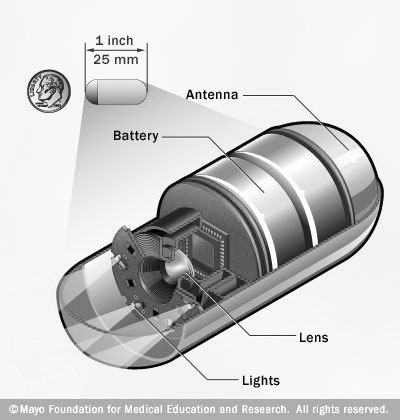
\includegraphics[]{capsule}
	\centering
	\caption{Kapsule \cite{capsule}\label{fig:capsule}}
\end{figure}

Ve většině případů je zapotřebí okolo osmi hodin \cite{diagnosing} pro průchod celým zažívacím traktem. Po dokončení celého procesu je kamera vyloučena z pacientova těla přirozenou cestou a již se nedá znovu použít. Vyšetření se provádí za účelem zjištění následujících nemocí (volně přeloženo z \cite{capsule}):

\begin{itemize}
\item Krvácení v zažívacím traktu - kapslová endoskopie může pomoci při určení příčiny krvácení.
\item Zánětlivé onemocnění střev - kapslová endoskopie může odhalit místa zánětu v tenkém střevě a tak pomoci diagnostikovat Crohnovu nemoc a další zánětlivá onemocnění.
\item Rakovina - kapslová endoskopie může identifikovat nádory v tenkém střevě, které by jinak byly těžko identifikovatelné. Kapslová endoskopie je občas prováděna se spojením s magnetickou rezonancí, protože magnetická rezonance může odhalit nádory ve stěně tenkého střeva.
\item Celiakie - některé malé studie tvrdí, že kapslová endoskopie může detekovat střevní změny spojené s celiakií - alergickou reakci po požití lepku - a může detekovat komplikace.
\item Polypy - lidé, kteří mají vrozenou polypózu, která může způsobovat polypy v tenkém střevě např. Peutz-Jeghersův syndrom, tak mohou využívat kapslovou endoskopii pro zobrazení polypů.
\end{itemize}

